\chapter{Introduction}\label{chap:introduction}


\section{Background and Motivation}\label{sec:motivation-and-background}

Recently, leaning-based control and reinforcement learning methods have been succeeding in more and more fields.
However, one of the most important concern with these methods is safety, or constraint satisfaction, of the system.
Usually, these methods do not incorporate system constraints in an explicit way, thus offering no guarantee of constraint satisfaction.

In \cite{wabersichPredictiveSafetyFilter2021a}, the authors proposed a model-based safety filter, which can be used to ensure safety of the system under arbitrary control inputs.
It has successfully kept safety in the controlling of pendulum and quadrotor in \cite{wabersichPredictiveSafetyFilter2021a}, as well as the controlling of Chronos \cite{carronChronosCRSDesign2022}, a radio controlled (RC) model vehicle, in \cite{tearlePredictiveSafetyFilterRacing2021}.
This safety filter is model-based, since it uses a model of the system to predict the future states and outputs.
Usually, this model comes from complicated modelling and system identification procedure.
This process is almost always time-consuming, computationally expensive, and requires expert knowledge.

In the meantime, data-driven predictive controllers have drawn more and more attention.
As introduced in \cite{willemsNotePersistencyExcitation2005}, the behavior of an LTI system can be fully captured by a rich enough dataset trajectory, which is commonly referred to as the \emph{fundamental lemma} of data-driven predictive control.
This result has also been extended to linear time invariant affine systems in \cite{martinelliDataDrivenAffine2022}, and to multiple dataset trajectories in \cite{vanwaardeMultiple2020}.

Based on this fundamental lemma, the prediction of future outputs of a system can be achieved without the need of a model.
This idea enlightened \emph{Data-enabled predictive control (DeePC)} in \cite{coulsonDataenabledPredictiveControl2019}, which is a data-driven predictive controller that directly use a dataset trajectory to predict future trajectory of the system.
In \cite{coulsonDataenabledPredictiveControl2019}, the authors also proposed a scheme of dealing with noise in both dataset trajectory and online observations: regularizing the auxiliary variables in the predictive controller.

This data-driven predictive controller has been proved effective in many fields.
In \cite{elokdaDataQuad2021}, the authors used DeePC to control a quadrotor, and the results show that the quadrotor can successfully track a reference point.
A sensitive analysis of hyperparameters in DeePC is also provided in \cite{elokdaDataQuad2021}, as well as suggestions of choosing these hyperparameters based on the empirical results.
In \cite{mullerDataDrivenQCR2022}, the authors used DeePC to model and control the noisy unknown dynamics of a quasi continuum manipulator.
The results show that DeePC can successfully deal with the noise and model discrepancy in the system, resulting in a dramatically reduced tracking error.
It is worth noticing that although the DeePC is originally designed for LTI systems, in \cite{elokdaDataQuad2021} and \cite{mullerDataDrivenQCR2022}, it is successfully applied to non-linear systems.

Apart from successful applications to real systems, there's also theoretical discussions regarding DeePC, for example the comparison between \emph{Direct} and \emph{Indirect} methods in DeePC, in \cite{dorflerBridgingDirectIndirect2023}.
The direct method, as the name suggests, deals with the data trajectory directly, while the indirect method accepts a mild preprocessing of the dataset.
It has been shown in \cite{dorflerBridgingDirectIndirect2023} that the regularized direct approach can be viewed as a convex relaxation of the indirect approach, and based on empirical results, the authors suggest indirect method in the case of variance errors such as output noise, and direct method in the case of bias errors such as model discrepancy.
In \cite{mattssonRegularizationDeePC}, different regularizers are proposed and compared, both in the context of DeePC and purely prediction problems.
The results reconfirm the conclusion in \cite{dorflerBridgingDirectIndirect2023}, that the indirect method outperforms direct method in the case of variance error.
In \cite{vanwingerdenInstrumentVar2022}, the authors discuss the relationship between direct DeePC, DeePC with instrumental variables, and the subspace identification method.
It is shown that the proposed DeePC with instrumental variables is equivalent to the subspace identification method.

Similar to the model predictive control (MPC), DeePC also faces the challenge of closed-loop guarantees, including recursive feasibility, constraint satisfaction and closed-loop stability.
In \cite{berberichDataDrivenRobust2021} and \cite{berberichStabilityInnerRobust2022IEEE}, the authors proved that DeePC with mild modifications has qualitative guarantees, namely with small enough noise bound, recursive feasibility and asymptotic stability hold in closed-loop.
The main drawback of these results is that no output constraints are considered.

In \cite{berberichRobustConstraintSatisfaction2020}, the authors proposed a constraint tightening scheme to ensure output constraints satisfaction in DeePC.
This scheme has the advantage of having rigorous guarantees, but the drawback of being conservative due to a generous estimation of prediction error.

There are also works for DeePC on non-linear systems.
In \cite{berberichLinearTrackingMPCData2022}, the authors provide a data-driven predictive controller for non-linear systems, which can be used to track a reference trajectory.
Recent online dataset is used to ensure that the system is linearized around current state.
Simulation results show that the proposed controller can successfully track a reference trajectory.

There are also works on a data-driven formulation that is different from DeePC, such as the one proposed in \cite{huangRobustDataEnabledPredictive2023}.
This scheme uses an auxiliary variable to take any possible error realization into account, and gives a tractable convex reformulation of the original problem.
Bound of open loop cost can be established, but the closed-loop guarantees and performance are yet to be discussed.

With the success and in-depth discussions of data-driven predictive control, it is natural to ask whether it is possible to design a data-driven predictive safety filter, which can be used to ensure safety of the system under arbitrary control inputs, and only requires dataset trajectories for off-line design.
Recently, in \cite{bajelaniDataDrivenSafetyFilter2023}, the authors proposed a data-driven safety filter for noise-free linear time invariant (LTI) systems.
But an extensive discussion of robust properties, applicability, and comparison of different formulations is yet to be done.
This thesis aims to fill this gap.

We first give a brief introduction of the background, motivation and preliminaries in \cref{chap:introduction}.
Then we introduce the nominal data-driven safety filter in \cref{chap:nominal-ddsf}, and show that it is equivalent to the model-based safety filter for noise-free LTI system.
As a result, guarantees including recursive feasibility and constraints satisfaction can be naturally established.
In \cref{chap:robust-ddsf-lti}, we incorporate the robust methods into data-driven safety filter, and provide comparison and analysis of different formulations, including the direct and indirect methods.
Numerical results are given to show that the proposed data-driven safety filter can successfully keep the system safe under arbitrary control inputs.
Comparison between direct and indirect methods show that indirect method is better for the safety filter, since it better decouples the prediction and input interfere.
In \cref{chap:non-linear-system}, we propose a data-driven prediction scheme for non-linear system, as well as a method of evaluating the quality of a certain dataset of trajectories.
Numerical example using a simple non-linear system is given to show that with the proposed data-driven prediction scheme, datasets with better quality yield better prediction performance.
Finally, in \cref{chap:test-chronos}, we test the proposed data-driven safety filter on Chronos, an RC model vehicle, and show that the safety filter can successfully keep the system safe under arbitrary control inputs.
We also propose a scheme of dataset collection for general systems, and show that this scheme can be used to collect a rich enough dataset for Chronos.


\section{Preliminaries}\label{sec:preliminaries}

First we introduce some basic notations used in this thesis.

{\renewcommand{\arraystretch}{1.5}%
\begin{center}
\begin{tabular}{ c|l }
    $\listinI{i}{j}$ & List of integers from $i$ to $j$, $\left\{ i, i+1, \dots, j \right\}$ \\
    \hline
    $\subseq{x}{i}{j}$ & Sequence of variables $\sequence{x}{k}{i}{j}$, with index from $i$ to $j$, $\left\{ x_i, x_{i+1}, \dots, x_j \right\}$ \\
    \hline
    $\norm{x}_P$ & $P$-norm of $x$, $\sqrt{\transpose{x} P x}$ \\
    \hline
    $A \otimes B$ & Kronecker product of real matrices $A$ and $B$ \\
    \hline
    $\Real^n$ & Set of real vectors of length $n$ \\
    \hline
    $\Real^{m \times n}$ & Set of $m$-by-$n$ real matrices \\
    \hline
    $\Real^{(m \times n)}$ & Set of real vectors of length $m \times n$ \\
    \hline
    $\ones{n}$ & All one vector of length $n$ \\
\end{tabular}
\end{center}
}

With a little abuse of notation, we also use $\subseq{x}{i}{j}$ to denote the column vector $\transpose{\begin{bmatrix}
    \transpose{x_i} & \transpose{x_{i+1}} & \ldots & \transpose{x_j}
\end{bmatrix}}$.
Also, we simply use $x$ to denote a sequence $\sequence{x}{k}{i}{j}$ if the index range $i$ and $j$ are clear from the context.

Without further notice, we always deal with discrete time invariant systems.
A general discrete time invariant system can be defined as:

\begin{definition}[Discrete Time Invariant Dynamic System]\label{def:dynamic-system}
    A dynamic system is defined by $\left(\Xset, \Uset, \Yset, f, g\right)$, where:

    $\Xset \subseteq \Real^n$ is the state constraint; $\Uset \subseteq \Real^m$ is the input constraint; $\Yset \subseteq \Real^p$ is the output constraint; $f: \Real^n \times \Real^m \rightarrow \Real^n$ is the state transition function; $g: \Real^n \times \Real^m \rightarrow \Real^p$ is the output function.

    For the rest of the Thesis, without further notice, we always assume the dimension of state, input and output are $n$, $m$ and $p$ respectively.
\end{definition}

Note that we define the state transition function and output function on the ambient linear space $\Real^n$ and $\Real^m$.
This is for the convenience of discussing \emph{trajectories} and \emph{safe trajectories} of the system.
We define trajectories of a dynamic system as:

\begin{definition}[Trajectory of a Dynamic System]\label{def:traj-dynamical-system}
    A list of input-output pairs $\sequence{u}{t}{i}{j}$ and $\sequence{y}{t}{i}{j}$, with $u_t \in \Real^m$ and $y_t \in \Real^p$, is called a trajectory of the dynamic system $\left(\Xset, \Uset, \Yset, f, g\right)$, if there exist $\sequence{x}{t}{i}{j}$, with $x_t = f\left(x_{t-1}, u_{t-1}\right)$, $x_t \in \Real^n$, and $y_t = g\left(x_t, u_t\right)$ hold for any $t$ in $\listinI{i+1}{j}$.
\end{definition}

Considering the constraints, we define the safe trajectories of a dynamic system as:

\begin{definition}[Safe Trajectory of Dynamic System]\label{def:safe-traj}
    A list of input-output pairs $\sequence{u}{t}{i}{j}$ and $\sequence{y}{t}{i}{j}$, with $u_k \in \Real^m$ and $y_t \in \Real^p$, is called a safe trajectory of the dynamic system $\left(\Xset, \Uset, \Yset, f, g\right)$, if there exist $\sequence{\tildeu}{t}{i}{\infty}$, $\sequence{\tildex}{t}{i}{\infty}$, and $\sequence{\tildey}{t}{i}{\infty}$ that satisfy:

    \begin{itemize}
        \item $\tildex_t = f\left(\tildex_{t-1}, \tildeu_{t-1}\right)$, $\tildey_t = g\left(\tildex_t, \tildeu_t\right)$ hold for any $t$ in $\left[i+1, \infty\right)$.
        \item $\tildex_t \in \Xset$, $\tildeu_t \in \Uset$, $\tildey_t \in \Yset$ hold for any $t$ in $\left[i, \infty\right)$.
        \item $\tildeu_t = u_t$, $\tildey_t = y_t$ hold for any $t$ in $\listinI{i}{j}$.
    \end{itemize}

\end{definition}

In another word, we view a trajectory $\sequence{u}{t}{i}{j}$ and $\sequence{y}{t}{i}{j}$ as safe, if it is possible to extend it
into an infinite trajectory of the system, and keep the constraints satisfied.

\begin{remark}\label{remark:safe-traj}
    As discussed later in \cref{remark:order-lag}, it is only possible to uniquely determine the state of the system with a long enough input-output trajectory.
    For example, the trajectory needs to be at least of length $l$ in the case of LTI system.

    But a shorter trajectory that is not long enough to determine the state of the system can still be safe, according to \cref{def:safe-traj}.
    In this case, the fact that \emph{observed a safe trajectory} does not imply that \emph{the system is safe}.
\end{remark}

Since we are dealing with data-driven methods, and the output $y_k$ of the system usually contains everything we can observe and care about for the system, for the rest of the Thesis, without further notice, we always assume $\Xset = \Real^n$
That is, there is no state constraint for the system.

As common in system theory, a dynamic system is linear if both the state transition function $f$ and output function $g$ are linear.
In our case, where the system is time invariant and the input, state and output are all finite dimensional real vectors, it is equivalent to say that both $f$ and $g$ can be represented by matrices:
There exist $A \in \RealMat{n}{n}$, $B \in \RealMat{n}{m}$, $C \in \RealMat{p}{n}$, $D \in \RealMat{p}{m}$, so that $f\left(x,u\right) = A x + B y$, $g\left(x, u\right) = C x + D u$.
We denote these matrices $A$, $B$, $C$, $D$ as the \emph{dynamic matrices} of the dynamic system.

A slightly more complicated family of systems is linear time invariant affine (LTI affine) systems, where $f$ and $g$ are affine functions.
In another word, apart from the dynamic matrices, we also have affine terms $a_f$ and $a_g$, respectively:
$f\left(x,u\right) = A x + B y + a_f$, $g\left(x, u\right) = C x + D u + a_g$.

By \emph{Kalman Decomposition}, any LTI system can be decomposed to observable/unobservable and controllable/uncontrollable parts.
As we always deal with the output of the system, the unobservable part is of no interest to us.

For simplicity, we accept the following definition of controllability:

\begin{definition}\label{def:lti-controllability}
    A pair of dynamic matrices $A$ and $B$ is controllable, if the controllability matrix $\mathcal{C} = \begin{bmatrix} B & A B & \ldots & A^{n-1} B \end{bmatrix}$ has full row rank.
    Where $n$ is the dimension of the state of the system.
\end{definition}

To ease the discussion in the Thesis, we also assume that the system is controllable.

As a reference to behavior system theory discussed in \cite{markovskyBehavioralSystemsTheory2021}, different dynamic matrices may give the same input-output response behavior $\mathscr{B}$.
Also, a certain behavior $\mathscr{B}$ can also be controllable or not.
Different dynamic matrices pairs $(A, B, C, D)$ and $\tilde{A}, \tilde{B}, \tilde{C}, \tilde{D}$, that result in the same input-output response behavior $\mathscr{B}$, are called different \emph{representations} of the same behavior.
And for a controllable behavior $\mathscr{B}$, we can always find a \emph{minimal realization} of the behavior, which is a dynamic matrices pair $(A, B, C, D)$ that is both controllable and observable.

Within the scope of this Thesis, we always assume the system behavior we are dealing with is controllable.
And when referring to the dynamic matrices of the system, we always refer to a minimal realization of the behavior.

We define the following invariants of a certain LTI system behavior $\mathscr{B}$:

\begin{definition}[Order and Lag of LTI System]\label{def:order-lag}
    For a controllable LTI system behavior $\mathscr{B}$ with a minimal realization $A$, $B$, $C$, $D$, we define the order $n$ of the system as the dimension of the state of the system, under this minimal realization.

    We define the lag of the system as the minimal integer $l$, that makes the observability matrix $\mathcal{O}_l = \transpose{\begin{bmatrix} \transpose{C} & \transpose{(C A)} & \ldots & \transpose{(C A^{l-1})} \end{bmatrix}}$ of full rank.
\end{definition}

\begin{remark}\label{remark:order-lag}
    Note that for any controllable LTI system behavior $\mathscr{B}$, the order and lag are well-defined, independent of the minimal realization, and $l \leq n$ holds.
    Also, the lag $l$ is also the minimal number of input-output pairs needed to uniquely determine the state of the system.
    See \cite{markovskyBehavioralSystemsTheory2021} for more details on behavioral system theory.
\end{remark}

In \cref{chap:nominal-ddsf} and \cref{chap:robust-ddsf-lti}, we will focus on linear time invariant (LTI) system.
While in \cref{chap:non-linear-system}, we touch upon linear time invariant affine systems and non-linear systems.

The \emph{Hankel Matrix} of certain depth constructed with a sequence of vectors is defined as:

\begin{definition}[Hankel Matrix]\label{def:hankel-matrix}
    For a sequence of vectors $\sequence{x}{k}{i}{j}$, with $x_k \in \Real^n$, the Hankel matrix of depth $L$ is defined as:

    \begin{equation*}
        \hankel{L}{\subseq{x}{i}{j}} = \begin{bmatrix}
            x_i & x_{i+1} & \ldots & x_{j-L+1} \\
            x_{i+1} & x_{i+2} & \ldots & x_{j-L+2} \\
            \vdots & \vdots & \ddots & \vdots \\
            x_{i+L-1} & x_{i+L} & \ldots & x_{j}
        \end{bmatrix} \in \RealMat{(n \times L)}{(j-i-L+2)}
    \end{equation*}

\end{definition}

Intuitively, each column of the Hankel matrix is the vertical stack of a sub-sequence with length $L$ of the original sequence. 
And all columns cover all possible length-$L$ sub-sequences of the original sequence.

The \emph{fundamental lemma} of data-driven predictive control, as introduced in \cite{willemsNotePersistencyExcitation2005}, states that the behavior of an LTI system can be fully captured by a \emph{rich enough} dataset trajectory.
Here rich enough is formally captured by the definition of \emph{persistently exciting} dataset trajectory:

\begin{definition}[Persistently Exciting]\label{def:persistently-exciting}
    We say a sequence of inputs $\sequence{u}{k}{0}{N-1}$ is persistently exciting of order $L$, if the Hankel matrix $\hankel{L}{\sequence{u}{k}{0}{N-1}}$ has full row rank (of rank $m \times L$).
\end{definition}

Then we can state the fundamental lemma as:

\begin{lemma}[Fundamental Lemma]\label{lemma:fundamental-lemma}
    Consider a controllable LTI system and a dataset trajectory of the system $\datasetSequence{u}{N}$ and $\datasetSequence{y}{N}$, with $\datasetSequence{u}{N}$ persistently exciting of order $L + n$, where $n$ is the order of the system.

    Then, $\subseq{u}{0}{L-1}$ and $\subseq{y}{0}{L-1}$ are a trajectory of the system if and only if there exist $\alpha$, which makes the following equation hold:
    \begin{equation*}
        \begin{bmatrix}
            \subseq{u}{0}{L-1} \\
            \subseq{y}{0}{L-1} \\
        \end{bmatrix} = \begin{bmatrix}
            \hankel{L}{\datasetSequence{u}{N}} \\
            \hankel{L}{\datasetSequence{y}{N}} \\
        \end{bmatrix} \alpha
    \end{equation*}
\end{lemma}

\Cref{lemma:fundamental-lemma} states that a rich enough dataset trajectory can represent the system behavior up to a certain length, so it shows the possibility of replacing a model of the system with only a dataset trajectory.

Also, as mentioned in \cref{remark:order-lag}, it is possible to uniquely determine the state of the system with a dataset trajectory of length that is larger than $l$.
By this intuition, we can define the input-output equilibrium of the system:

\begin{definition}[Input-Output Equilibrium]\label{def:input-output-equilibrium}
    An input-output pair $\left(\us, \ys\right)$ is called an input-output equilibrium of the system, if $\left\{\us\right\}_{t=0}^{l}$ and $\left\{\ys\right\}_{t=0}^{l}$ is a trajectory of the system.
    Where $l$ is the lag of the system.
\end{definition}

The intuition is that, if a pair $\left(\us, \ys\right)$ satisfies \cref{def:input-output-equilibrium}, then $\left\{\us\right\}_{t=0}^{\infty}$ and $\left\{\ys\right\}_{t=0}^{\infty}$ is a trajectory of the system.
Which means the system can stay at the input-output equilibrium forever.

\begin{remark}\label{remark:safe-equilibrium}
    According to \cref{def:safe-traj}, if $\left(\us, \ys\right)$ is an input-output equilibrium of the system, and $\us \in \Uset$, $\ys \in \Yset$ hold, then $\constantSequence{\us}{0}{L-1}$ and $\constantSequence{\ys}{0}{L-1}$ is also a safe trajectory for the system with any length $L$.
\end{remark}

Finally, we give a brief introduction to predictive safety filter, as introduced in \cite{wabersichPredictiveSafetyFilter2021a}.
As said in \cref{sec:motivation-and-background}, predictive safety filter aims at keeping the system safe under arbitrary control inputs.
For now let's assume we have full observation of the system, which means $g(x,u) = x$.
With a general leaning based controller, which can give any inputs, The overall data flow can be seen in \cref{img:predictive-safety-filter}.
A safety filter is attached to the system, which takes input from the learning based controller, the state of the system, and gives out a safe input to the system.

\begin{figure}[ht]
    \centering
    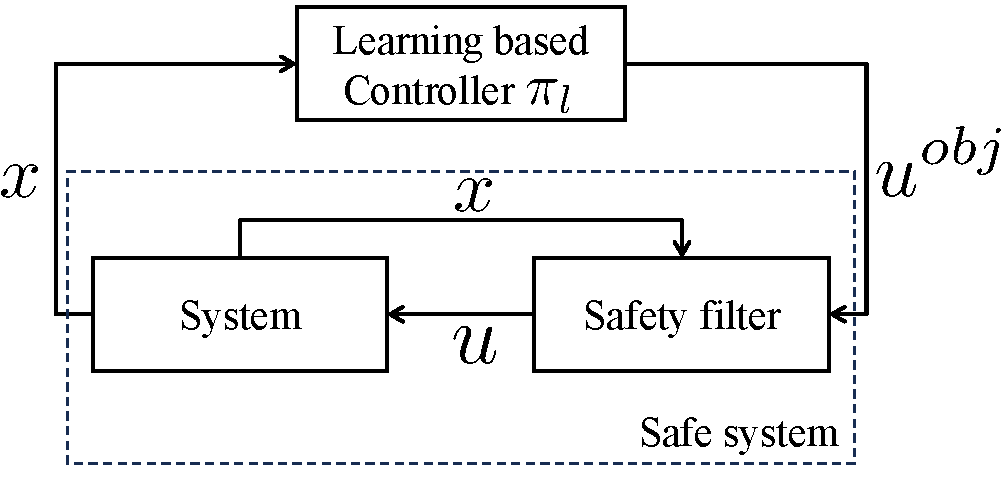
\includegraphics[width=0.7\textwidth]{\imagedir/predictiveSF.pdf}
    \caption{Predictive Safety Filter}
    \label{img:predictive-safety-filter}
\end{figure}

With a dynamic system $\left(\Xset, \Uset, \Yset, f, g\right)$, the predictive safety filter solves the following optimization problem:

\begin{subequations}
\label{eq:state-based-safety-filter} 
\begin{align}
    \min_{\substack{\bar{u}, \bar{x}}} \quad & \norm{u_{0} - u^{\text{obj}}}_R  \label{eq:state-based-safety-filter-cost} \\
    \textrm{s.t.} \quad & 
    \bar{x}_{k} = f(\barx_{k-1}, \baru_{k-1}) \quad k \in \left[1, L-1\right] \label{eq:state-based-safety-filter-dynamics} \\
    & 
    \barx_0 = x_t \label{eq:state-based-safety-filter-initial}\\
    & 
    \barx_{L-1} \in \Sset_f \label{eq:state-based-safety-filter-terminal} \\
    &
    \bar{u}_k \in \Uset, \quad k \in \left[0, L-1\right] \label{eq:state-based-safety-filter-input}\\
    &
    \bar{x}_k \in \Xset, \quad k \in \left[0, L-1\right] \label{eq:state-based-safety-filter-output}
\end{align}
\end{subequations}

Within the scope of this thesis, we always use plain variables with subscripts to denote online observation and closed loop response, and use variables with a bar on top to denote the variables of optimization problems.
When it is necessary, we also use brackets to denote the time step of the optimization problem, for example $\barx(t)$ is the optimization variable of the system state at time step $t$.
Also, we denote the optimal solution by $(-)^*$, for example $u^*(t)$ represents the optimal solution at time step $t$, and candidate solution by a hat on top, for example $\hatx(t+1)$ represents the candidate solution for time step $t+1$.

Where $L$ is the prediction horizon, $x_t$ is the current state of the system, $\uObj$ is current control input supposed by the learning based controller, $R$ is the weighting matrix used to examine the distance between the actual input and the desired input.

$\Sset_f$ is a safe terminal set of the system, we refer to an in-detail discuss in Assumption 4.2 in \cite{wabersichPredictiveSafetyFilter2021a}.
Intuitively, it is a set of states, that there exists a safe feedback controller, which can keep the system within constraints for all future time steps if the system starts from this set.

When working with predictive style controllers, it is common to use \emph{one-step receding horizon} scheme.
This means at each time step the optimization problem is solved, and only the first input of the optimal solution is applied to the system.
Then the optimization problem is solved again at the next time step, with the new state of the system and the new desired input.
Later in \cref{chap:robust-ddsf-lti}, we will introduce a slightly different \emph{multi-step receding horizon} scheme, which is needed for the robustness analysis, as discussed in \cite{berberichDataDrivenRobust2021}.

As discussed in \cite{wabersichPredictiveSafetyFilter2021a}, recursive feasibility and closed-loop constraint satisfaction can be proved for this safety filter, following the one-step receding horizon scheme.
In another word, if the optimization problem is feasible at time step $0$, then the constraint will be satisfied and the optimization problem will be feasible at all future time steps $t \geq 0$.
